\chapter{Results}
\label{ch:results}

{This chapter is a template. The analysis has not been run, so it contains no
findings yet. Empty cells and figures mark where each result goes.}

\section{Dataset overview}
\label{sec:results-overview}

Table~\ref{tab:dataset} summarizes the analyzed snapshot.

\begin{table}[htbp]
  \centering
  \caption{Overview of the analyzed snapshot}
  \label{tab:dataset}
  \begin{tabular}{lrr}
    \toprule
    & CC & FIPS~140 \\
    \midrule
    Certificates & -- & -- \\
    Documents processed & -- & -- \\
    Documents with usable text & -- & -- \\
    Date range & -- & -- \\
    \bottomrule
  \end{tabular}
\end{table}

\section{Extraction quality}
\label{sec:results-quality}

Because the remaining results rest on the extraction, its measured quality is
reported first (Table~\ref{tab:quality}).

\begin{table}[htbp]
  \centering
  \caption{Extraction quality on the annotated sample}
  \label{tab:quality}
  \begin{tabular}{lrr}
    \toprule
    Method & Precision & Recall \\
    \midrule
    Regular expressions & -- & -- \\
    Regular expressions and model & -- & -- \\
    \bottomrule
  \end{tabular}
\end{table}

\section{RQ1: Footprint of OpenSSL and its forks}
\label{sec:results-rq1}

{Describe the prevalence per library and scheme, the trends over time, and the
vendor concentration.}

\begin{table}[htbp]
  \centering
  \caption{Certificates with a dependency on each library, by evidence level}
  \label{tab:prevalence}
  \begin{tabular}{lrrrrrr}
    \toprule
    & \multicolumn{3}{c}{CC} & \multicolumn{3}{c}{FIPS~140} \\
    Library & E1 & E2 & E3 & E1 & E2 & E3 \\
    \midrule
    OpenSSL   & -- & -- & -- & -- & -- & -- \\
    LibreSSL  & -- & -- & -- & -- & -- & -- \\
    BoringSSL & -- & -- & -- & -- & -- & -- \\
    AWS-LC    & -- & -- & -- & -- & -- & -- \\
    quictls   & -- & -- & -- & -- & -- & -- \\
    \bottomrule
  \end{tabular}
\end{table}

\begin{figure}[htbp]
  \centering
  \fbox{\parbox[c][4cm][c]{0.8\textwidth}{\centering Placeholder: stacked area
    chart of library prevalence per certification year.}}
  \caption{Library prevalence over time (placeholder)}
  \label{fig:prevalence}
\end{figure}

\begin{figure}[htbp]
  \centering
  \fbox{\parbox[c][4cm][c]{0.8\textwidth}{\centering Placeholder: bipartite
    graph of vendors and libraries.}}
  \caption{Vendor and library dependency graph (placeholder)}
  \label{fig:graph}
\end{figure}

\subsection{Undeclared OpenSSL API usage}
\label{sec:results-api-detection}

The keyword extraction in sec-certs records OpenSSL only when a document names
the library. To find certificates that use OpenSSL without naming it, the texts
of all certificates without OpenSSL in their keywords were scanned for OpenSSL
API names. These are the 5,116 functions from the OpenSSL~3.3 manual whose
names start with a known OpenSSL prefix such as \texttt{SSL\_}, \texttt{EVP\_}
or \texttt{BIO\_}, together with header paths (\texttt{openssl/\dots}),
library files (\texttt{libcrypto}, \texttt{libssl}) and core types such as
\texttt{SSL\_CTX}. For CC the report, the Security Target and the certificate
were scanned, and for FIPS~140 the Security Policy.

API names alone do not prove that OpenSSL is used, because its forks and
API-compatible libraries share them. Each matching certificate was therefore
assigned to one class, checked in this order:
\begin{compactenum}
  \item \emph{OpenSSL derivative}: a derivative library (BoringSSL, AWS-LC,
    LibreSSL, RSA BSAFE or wolfSSL) is named in the text, BoringSSL, LibreSSL
    or wolfSSL is declared in the keywords, or the text includes the header
    \texttt{openssl/\allowbreak service\_indicator.h}, which exists only in
    BoringSSL and AWS-LC.
  \item \emph{OpenSSL named, not in keywords}: the text names OpenSSL, but the
    keyword extraction did not record it.
  \item \emph{API names only}: OpenSSL API names appear, but no library is
    named.
\end{compactenum}

Table~\ref{tab:api-detection} shows the result. The scan found 250
certificates, 108 CC and 142 FIPS~140. Almost half of them (112) turned out to
use a derivative rather than OpenSSL itself. All 45 CC derivatives are
BoringSSL. The 67 FIPS derivatives are BoringSSL (29), RSA BSAFE (18), BoringSSL
or AWS-LC identified only through \texttt{service\_indicator.h} (12) and AWS-LC
(8). Only 16 certificates name OpenSSL in their text without it appearing in the
keywords. This does not measure the recall of the keyword extraction in
general, because certificates that name OpenSSL without using any of its API
names were not part of the scan. The largest
class, 122 certificates, contains API names but no library name. These are
candidates for undeclared OpenSSL use, but they need manual review, because the
names can also come from another API-compatible library.

\begin{table}[htbp]
  \centering
  \caption{Certificates using OpenSSL API names without OpenSSL in their
    keywords, by class}
  \label{tab:api-detection}
  \begin{tabular}{lrrr}
    \toprule
    Class & CC & FIPS~140 & Total \\
    \midrule
    OpenSSL derivative             &  45 &  67 & 112 \\
    OpenSSL named, not in keywords &   9 &   7 &  16 \\
    API names only                 &  54 &  68 & 122 \\
    \midrule
    Total                          & 108 & 142 & 250 \\
    \bottomrule
  \end{tabular}
\end{table}

\section{RQ2: Gap between upstream releases and certification}
\label{sec:results-rq2}

{Report the distribution of the lag from Equation~\ref{eq:lag} and the release
distance, separately for initial certificates, maintenance or re-validation events,
and FIPS provider certificates.}

\begin{table}[htbp]
  \centering
  \caption{Certification lag in days, by scheme and event type}
  \label{tab:lag}
  \begin{tabular}{lrrrr}
    \toprule
    Group & $n$ & Median & Q1 & Q3 \\
    \midrule
    CC, initial certificate & -- & -- & -- & -- \\
    CC, maintenance & -- & -- & -- & -- \\
    FIPS~140-2, initial validation & -- & -- & -- & -- \\
    FIPS~140-3, initial validation & -- & -- & -- & -- \\
    FIPS, re-validation & -- & -- & -- & -- \\
    \bottomrule
  \end{tabular}
\end{table}

\begin{figure}[htbp]
  \centering
  \fbox{\parbox[c][4cm][c]{0.8\textwidth}{\centering Placeholder: timeline of
    upstream OpenSSL releases against the certificates that use them.}}
  \caption{Upstream releases and dependent certificates (placeholder)}
  \label{fig:timeline}
\end{figure}

\section{RQ3: Integration into sec-certs workflows}
\label{sec:results-rq3}

{Describe the resulting workflow, its integration points with sec-certs,
whether the analysis was successfully regenerated from the snapshot, and the model
cost.}

\section{Cryptographic algorithms by country}
\label{sec:results-country}

This section groups the cryptographic algorithms that certificates mention by
country. For CC the country is the certification scheme. FIPS~140 records have
no country field, so the vendor's headquarters country is used instead. It was
assigned by hand for the vendors with the most certificates, which leaves 25\,\%
of the FIPS certificates with an unknown country. Those certificates are left
out of the country comparisons. Each value is the share of a country's
certificates that mention the algorithm at least once. Countries with fewer than
50 certificates are not shown. In the figures restricted to one product
category or one issue period, the threshold is 30 certificates in that subset.

\subsection{Algorithm usage}
\label{sec:results-country-usage}

Figures~\ref{fig:cc-country-heatmap} and~\ref{fig:fips-country-heatmap} show the
30 algorithms with the highest average share. Most countries share a common core
of AES, SHA-2, SHA-1, MAC constructions (HMAC and CMAC, which the keyword
extraction does not distinguish) and Diffie--Hellman. The clearest national signal is
Korea: 37\,\% of Korean CC certificates mention SEED and 26\,\% mention ARIA,
against 1.7\,\% and 0.7\,\% of all CC certificates. In FIPS~140, a country often
stands for only a few vendors. The UK figures, for example, reflect almost
entirely nCipher, which explains Serpent and Twofish at 45\,\% and RIPEMD at
84\,\%.

\begin{figure}[htbp]
  \centering
  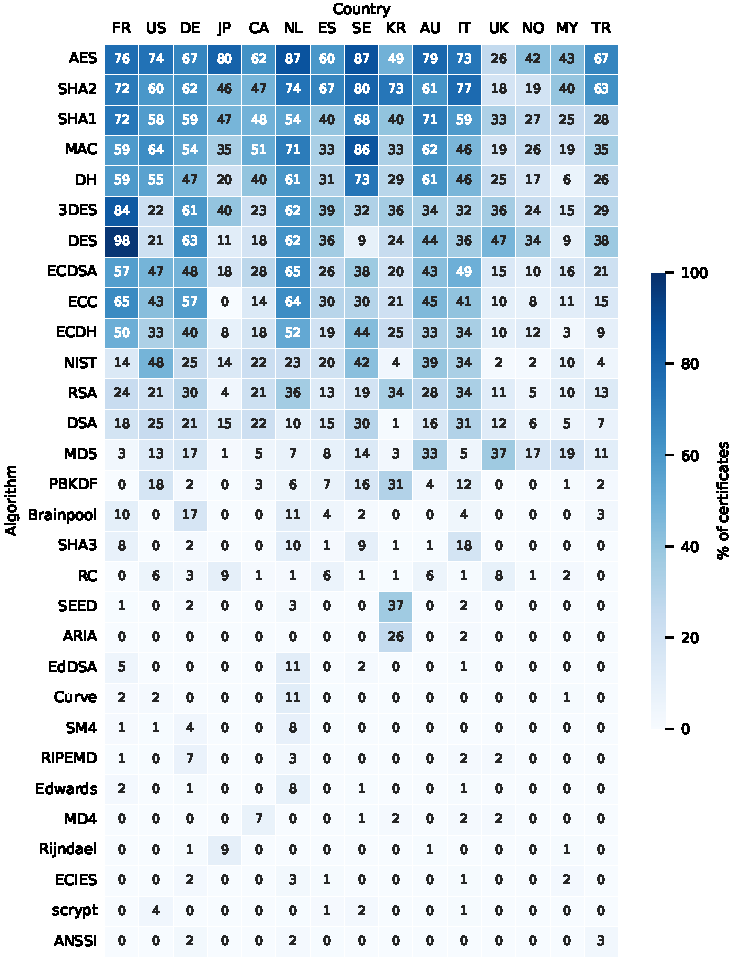
\includegraphics{cc_country_algorithm_heatmap}
  \caption{Share of CC certificates mentioning each algorithm, by scheme}
  \label{fig:cc-country-heatmap}
\end{figure}

\begin{figure}[htbp]
  \centering
  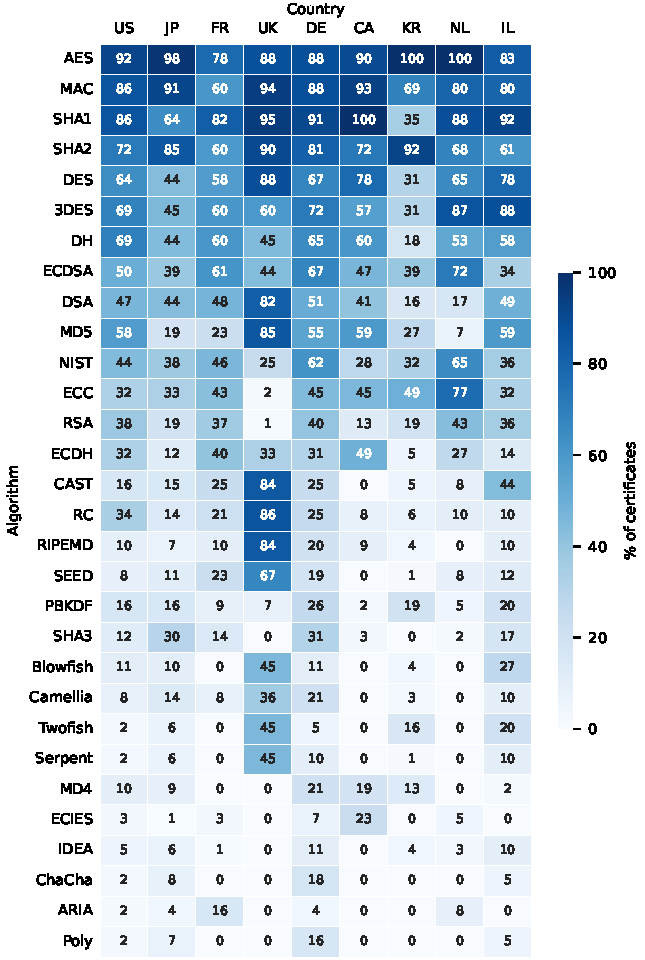
\includegraphics{fips_country_algorithm_heatmap}
  \caption{Share of FIPS~140 certificates mentioning each algorithm, by vendor
    country}
  \label{fig:fips-country-heatmap}
\end{figure}

\subsection{Product category and issue period}
\label{sec:results-country-confounders}

Two confounders affect the CC comparison. First, schemes certify different
product mixes: 89\,\% of French certificates are smart cards, while the largest
group of US certificates are network devices (34\,\%) and none are smart cards.
Figures~\ref{fig:cc-country-smartcards} and~\ref{fig:cc-country-network}
therefore compare the schemes within each of these two categories. Second,
schemes were active in different periods. UK certificates run from 1998 to 2017
with a median of 2006, while the median for the Netherlands is 2023.
Figures~\ref{fig:cc-country-older} and~\ref{fig:cc-country-recent} split the
certificates at 2017, the median issue year across the dataset.

The split separates the two effects. French DES mentions stay at 96--99\,\% in
both periods, so they follow from the smart-card product mix rather than from
the era. In contrast, US DES mentions drop from 34\,\% to 9\,\%. The low AES and
SHA-2 shares of the UK scheme are an era effect, because the UK appears only in
the earlier period. The Korean national ciphers are a current preference rather
than a legacy one: SEED rises from 32\,\% to 41\,\% and ARIA from 7\,\% to
44\,\% after 2017.

\begin{figure}[htbp]
  \centering
  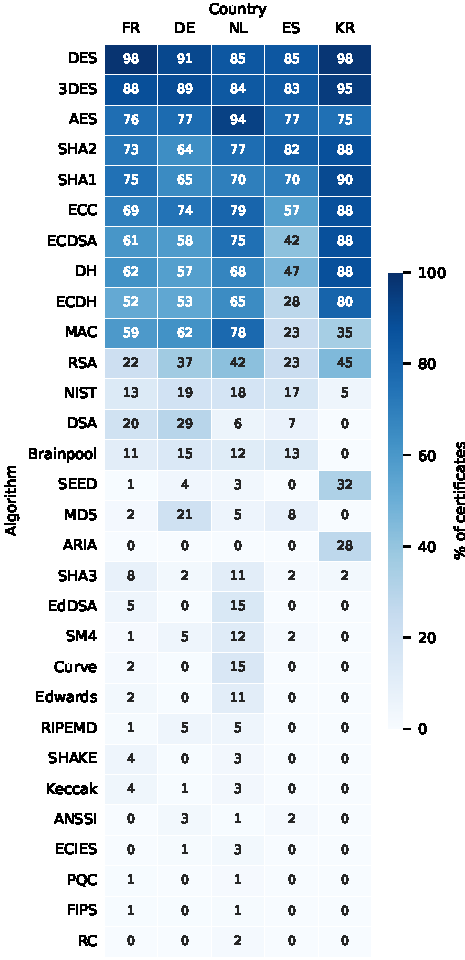
\includegraphics{cc_country_algorithm_heatmap_smartcards}
  \caption{Share of CC smart card certificates mentioning each algorithm, by
    scheme}
  \label{fig:cc-country-smartcards}
\end{figure}

\begin{figure}[htbp]
  \centering
  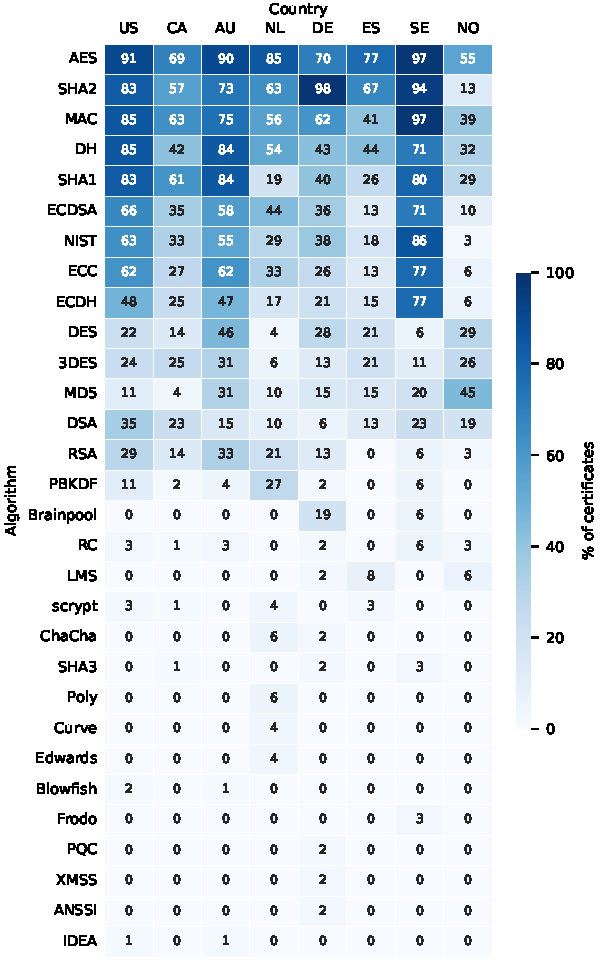
\includegraphics{cc_country_algorithm_heatmap_network}
  \caption{Share of CC network device certificates mentioning each algorithm,
    by scheme}
  \label{fig:cc-country-network}
\end{figure}

\begin{figure}[htbp]
  \centering
  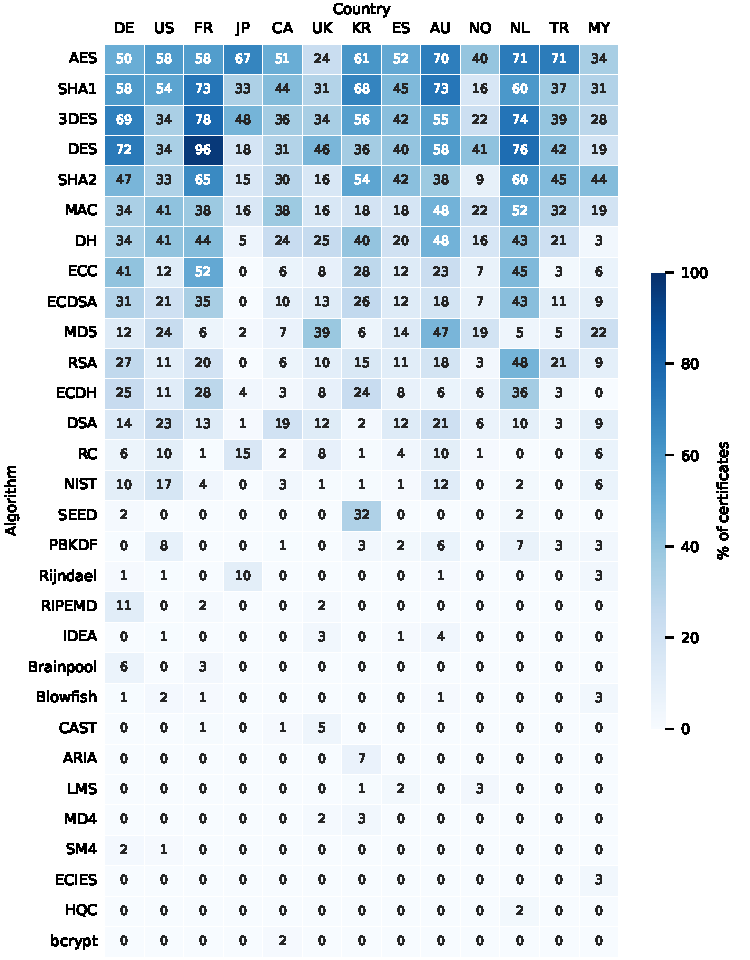
\includegraphics{cc_country_algorithm_heatmap_older}
  \caption{Share of CC certificates issued before 2017 mentioning each
    algorithm, by scheme}
  \label{fig:cc-country-older}
\end{figure}

\begin{figure}[htbp]
  \centering
  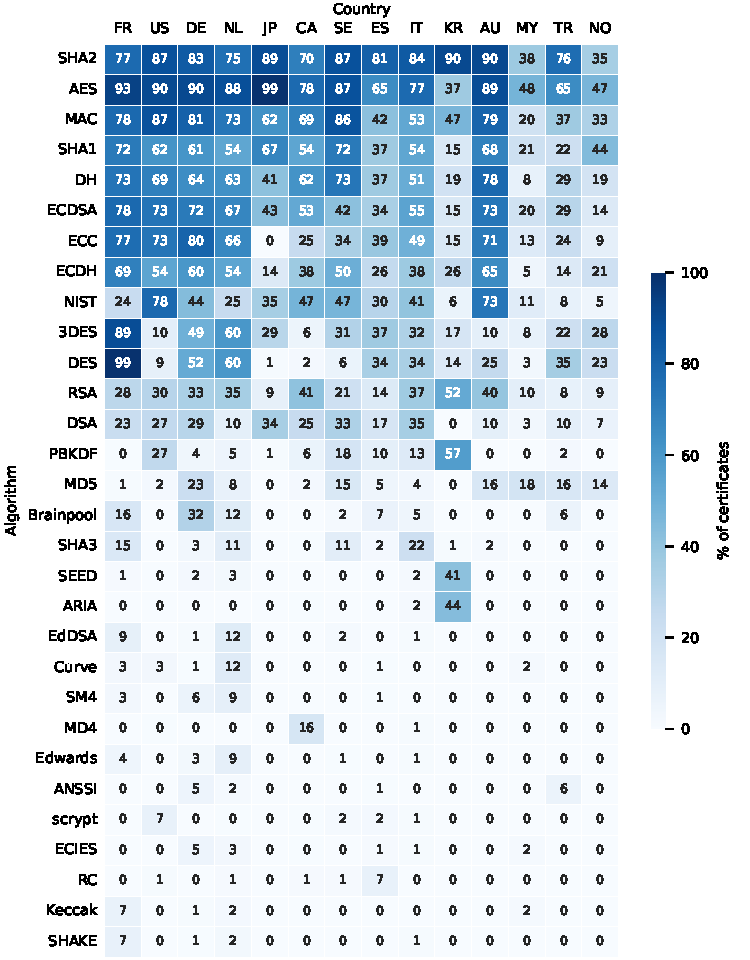
\includegraphics{cc_country_algorithm_heatmap_recent}
  \caption{Share of CC certificates issued in 2017 or later mentioning each
    algorithm, by scheme}
  \label{fig:cc-country-recent}
\end{figure}

\subsection{OpenSSL by country}
\label{sec:results-country-openssl}

A certificate counts as OpenSSL-based when OpenSSL appears among the crypto
libraries detected in its documents. This applies to 1,196 of 6,819 CC
certificates and 968 of 5,423 FIPS~140 certificates.
Figure~\ref{fig:openssl-country} shows how this share differs by country. Among
CC schemes it ranges from 53\,\% in Sweden to 1.4\,\% in France. Part of this
gap is product mix again, so the second panel restricts CC to network devices,
where Sweden reaches 83\,\% (this panel includes countries with at least 30
network device certificates). Among FIPS vendor countries, Germany (26\,\%) and
Japan (21\,\%) lead.

Figure~\ref{fig:openssl-gap} compares the algorithms mentioned by OpenSSL-based
certificates with those mentioned by other certificates. OpenSSL-based documents
tend to list the whole OpenSSL algorithm catalogue, so they mention almost every
algorithm more often. The elliptic-curve algorithms show the largest gap. ECDSA
and the NIST curves differ by about 40 percentage points in both schemes, and
ECDH does so among CC network devices, but only by 20 points in FIPS~140, where
DSA and Diffie--Hellman show larger gaps (about 33 points).
Among CC network devices, 3DES is the clearest exception: OpenSSL-based
certificates mention it 9 percentage points less often.

\begin{figure}[htbp]
  \centering
  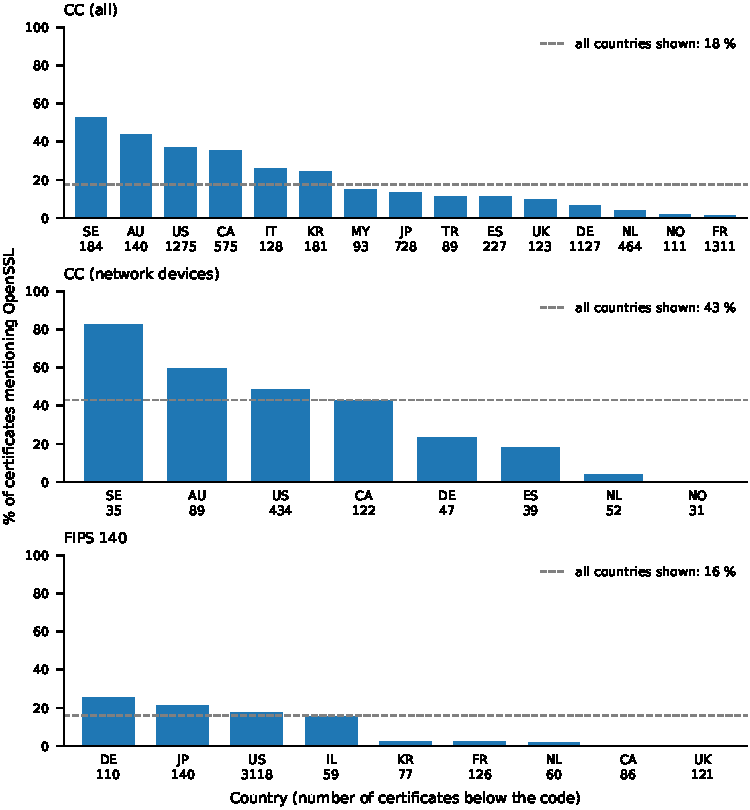
\includegraphics{openssl_share_by_country}
  \caption{Share of certificates mentioning OpenSSL, by country}
  \label{fig:openssl-country}
\end{figure}

\begin{figure}[htbp]
  \centering
  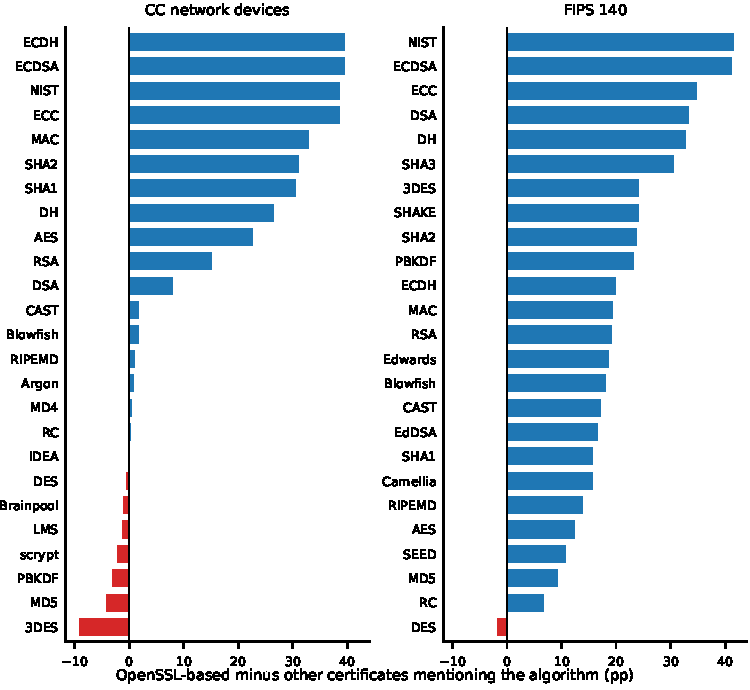
\includegraphics{openssl_algorithm_gap}
  \caption{Difference between the share of OpenSSL-based and other certificates
    mentioning each algorithm, for CC network devices and FIPS~140}
  \label{fig:openssl-gap}
\end{figure}

OpenSSL also ships several national ciphers: SEED and ARIA (Korea), Camellia
(Japan) and SM4 (China). Table~\ref{tab:national-ciphers} shows how often the
certificates that mention each cipher are OpenSSL-based, compared with all
certificates in the same scope. In FIPS~140, outside the home country, SEED,
ARIA, Camellia and SM4 mentions are OpenSSL-based about twice as often as the
baseline (26--38\,\% against about 16\,\%), so OpenSSL is a likely source of
these mentions. Korean CC certificates show the opposite: those mentioning SEED
or ARIA are less often OpenSSL-based than Korean certificates overall, which
suggests that Korean vendors use their own implementations. Groups with fewer
than ten certificates are too small to interpret. In the table, $n$ is the
number of certificates in the scope that mention the cipher, \enquote{OpenSSL}
is the percentage of them that are OpenSSL-based, and \enquote{Baseline} is the
percentage of all certificates in the scope that are OpenSSL-based.

\begin{table}[htbp]
  \centering
  \caption{OpenSSL-based certificates among those mentioning a national cipher}
  \label{tab:national-ciphers}
  \begin{tabular}{lllrrr}
    \toprule
    Scheme & Cipher (home) & Scope & $n$ & OpenSSL & Baseline \\
    \midrule
    CC   & SEED (KR)       & home      &  67 &  19.4 & 24.3 \\
    CC   & SEED (KR)       & elsewhere &  49 &   4.1 & 17.4 \\
    CC   & ARIA (KR)       & home      &  47 &  12.8 & 24.3 \\
    CC   & ARIA (KR)       & elsewhere &   4 & 100.0 & 17.4 \\
    CC   & Camellia (JP)   & elsewhere &   4 &   0.0 & 18.0 \\
    CC   & SM4 (CN)        & elsewhere & 111 &  18.9 & 17.5 \\
    CC   & GOST (RU)       & elsewhere &   1 &   0.0 & 17.5 \\
    \midrule
    FIPS & SEED (KR)       & home      &   1 &   0.0 &  2.6 \\
    FIPS & SEED (KR)       & elsewhere & 428 &  26.4 & 16.5 \\
    FIPS & ARIA (KR)       & elsewhere &  87 &  26.4 & 16.5 \\
    FIPS & Camellia (JP)   & home      &  19 &  63.2 & 21.4 \\
    FIPS & Camellia (JP)   & elsewhere & 331 &  36.0 & 16.0 \\
    FIPS & SM4 (CN)        & home      &   4 &   0.0 & 35.7 \\
    FIPS & SM4 (CN)        & elsewhere &  58 &  37.9 & 16.1 \\
    FIPS & GOST (RU)       & elsewhere &   7 &  14.3 & 16.2 \\
    \bottomrule
  \end{tabular}
\end{table}
